\chapter{Set Theory and Counting Techniques}

Two approaches of the concept of probability will introduced lately in this notes: The classical probability 
and the experimental probability. The sample space of probability theory is developed using the 
foundation of set theory.

In set theory, the number of elements in a set has a special name. It is
 called the \textbf{cardinality} of the set. In this notes we write $\hash(A)$ to represent the 
 cardinality of the set $A$.

\section{Notion of sets}

Set is a basic term in mathematics. One can think of a set to be a \textit{class} or \textit{collection}.

\begin{definition}[Sets]
    A set is a collection of objects called elements or numbers.
\end{definition}

\begin{definition}[Empty set]
    The empty set is the set with no elements, denoted as $\varnothing$ or $\{\}$.
\end{definition}

\begin{example}
    Throughout this notes, we are using the following number systems.
    \begin{itemize}
        \item The set of all nonzero positive integers, known as natural numbers
        \[ \mathbb{N} = \{1, 2, 3, \ldots \}. \]
        \item The set of all integers, regardless positive or negative,
        \[
            \mathbb{Z} = \{ \ldots, -3, -2, -1, 0, 1, 2, 3, \ldots \}.
        \]
        \item The set of all rational numbers, the numbers that can be express as 
            ratio of two integers
        \[
            \mathbb{Q} = \left\{ \frac{p}{q} : p, q \in \mathbb{Z} \quad \text{with } q \neq 0 \right\}
        \]
        \item The set of all real numbers, 
        \[
            \mathbb{R} = \{ \mathbb{Q} \text{ along with all irrational numbers such as } \sqrt{2}, \pi, e, \ldots \}.
        \]
    \end{itemize}
\end{example}

\begin{definition}[Subsets]
    A set $A$ is a subset of $B$, $A \subset B$, if $a \in A \implies a \in B$.
\end{definition}

\begin{example}
    What is the cardinality of each of the following sets?
    \begin{enumerate}
        \item $\varnothing$.
        \item $\{ \varnothing \}$.
        \item $A = \{ {\color{red}\heartsuit},  \{{\color{orange!50!white} \clubsuit } \} , \{{\color{red}\heartsuit}, \{{\color{red}\heartsuit}\} \} \}.$
        \item $B = \{ x | x \text{ is an integer such that } 2x^2 + 3x - 2 = 0 \}.$
    \end{enumerate}
\end{example}
\begin{solution}
    \begin{enumerate}
        \item Certainly, $\hash(\varnothing) = 0$.
        \item This is a set consists of one element $\varnothing$, thus $\hash(\{ \varnothing \}) = 1$.
        \item The set $A$ consists of three elements which are \fbox{${\color{red}\heartsuit}$}, \fbox{$\{{\color{orange!50!white} \clubsuit } \}$}, 
        and \fbox{$\{{\color{red}\heartsuit}, \{{\color{red}\heartsuit}\} \}$}. So $\hash(A) = 3$.
        \item Solving the quadratic equation,
            \begin{align*}
                2x^2 + 3x - 2 = 0 &\implies (2x - 1)(x + 2) = 0\\
                &\implies x = -2 \quad \text{ or } \quad x = \frac{1}{2}.
            \end{align*}
        Only $x = -2$ is integer. Thus $\hash (B) = \hash (\{-2\}) = 1$.
    \end{enumerate}
\end{solution}

\begin{definition}[Power Set]
    If $A$ is a set, then $\mathcal{P}(A) = \{B : B \subset A\}$.
\end{definition}

\begin{example}
    If $A = \varnothing$, then $\mathcal{P}(A) = \{ \varnothing \}$. The power set has only one single element, that is the 
    empty set itself.
\end{example}

\section{Set Operations}

\begin{theorem}[Properties of set union and intersect]
    For any three sets, $A$, $B$, and $C$.
    \begin{enumerate}[label=S\arabic*]
    \item \textbf{[Commutativity]}\quad  \[A \cup B = B \cup A,\] \[A \cap B = B \cap A.\]
    \item \textbf{[Associativity]}\quad   \[A \cup (B \cup C) = (A \cup B) \cup C,\] \[A \cap (B \cap C) = (A \cap B) \cap C,\]
    \item \textbf{[Distributive]}\quad   \[A \cap (B \cup C) = (A \cap B) \cup (A \cap C),\] \[A \cup (B \cap C) = (A \cup B) \cap (A \cup C)\]
    \item \textbf{[DeMorgan's law]}\quad   \[(A \cup B)^c = A^c \cap B^c, \] \[(A \cap B)^c = A^c \cup B^c\]
    \end{enumerate}
\end{theorem}

\subsection{Proof by induction}

Mathematical induction is a proof technique for proving that a statement is true for all natural numbers. It works by first proving a base case (the first natural number, often 1) 
and then proving an inductive step which shows that if the statement holds for some arbitrary integer $k$. 

\begin{figure}[ht]
    \centering
    \makebox[\textwidth]{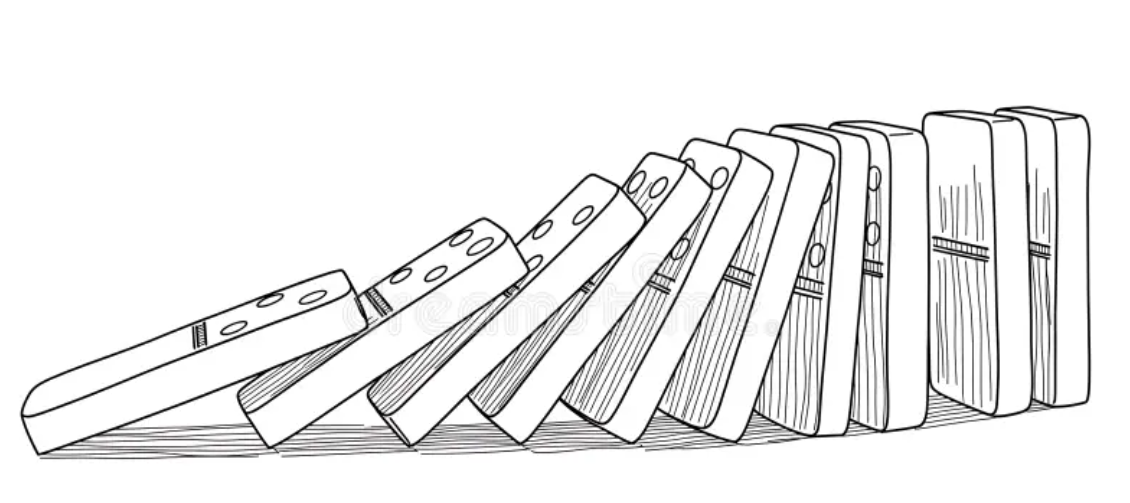
\includegraphics[width=0.4\paperwidth]{./images/domino.png}}
\end{figure}


\begin{theorem}[Mathematical Induction]
    Let $P(n)$ be a statement relies on $n \in \mathbb{N}$. Assume that
    \begin{enumerate}
    \item (Base case) $P(1)$ is true.
    \item (Induction step) If $P(m)$ is true, then $P(m+1)$ is true.
    \end{enumerate}
\end{theorem}
\begin{proof}
    Let 
    \[
        S = \{ n \in \mathbb{N} : P(n) \text{ is not true} \}.
    \]
    We want to show $S$ is empty. We will show this by contradiction.

    \textbf{Intuition:} By assuming $S \neq \varnothing$ and derive a false 
    statement. The rules of logic $p \rightarrow q$ (If $p$ then $q$) say that $S \neq \varnothing$ is false.

    \textit{For the sake of contradiction}, suppose $S \neq \varnothing$. By Well Ordering Principle of 
    natural numbers, $S$ has a least element $x \in S$. Given that the basis step $P(1)$ is true, 
    then $1 \notin S \implies x \neq 1$. In particular, $x > 1$.

    Since $x$ is the least element of $S$, and $x - 1 < x$, thus $x -1 \notin S$. From $S \neq \varnothing$, 
    we are now arriving to the conclusion that $\exists x \in \mathbb{N}$ such that $x \in S$ and $x \notin S$ 
    at the same time. This is a contradiction. Therefore $S$ must be empty.
\end{proof}


\section{Counting Techniques}

\begin{theorem}[Multiplication rule of counting]
    If a choice consists of $k$ steps, of which the first can be made in $n_1$ ways, for each of these the second can be made in $n_2$ 
    ways and so on. For each of these $k$-th can be made in $n_k$ ways, then the whole choice can be made in 
    \[
        n_1 \times n_2 \times \cdots \times n_k
    \]
    ways.
\end{theorem}
\begin{proof}
    In the notion of set theory, we use $S_i$ to represent the set of outcomes for the $i$-th step for all $i = 1, 2, \ldots, k$. 
    Then $\hash (S_i) = n_i$. The set of outcomes for the entire job is the Cartesian product 
    \begin{equation}
        S_1 \times S_2 \times \cdots \times S_k = \{ (s_1, s_2, \ldots, s_k) : s_i \in S_i, \quad 1 \leq i \leq k \}.
    \end{equation}
    Thus, we just need to show that the number of outcomes is equal to the product of number of choices for each step. That is,
    \begin{equation}
        \hash (S_1 \times S_2 \times \cdots \times S_k) = \hash S_1 \cdot \hash S_2 \cdot \cdots \cdot \hash S_k
    \end{equation}

    \textbf{[Basis Step]} By Theorem 1.2.5, we have $\hash(S_1 \times S_2) = \hash(S_1) \times \hash(S_2)$. Thus, the property
    is true for $n = 2$.

    \vspace*{0.5em}
    \textbf{[Induction Hypothesis]}
    Suppose
    \[
        \hash(S_1 \times S_2 \times \cdots \times S_k) = \hash(S_1) \cdot \hash(S_2) \cdots \hash(S_k)
    \]
    for $k = 2, 3, \cdots, n$.

    \vspace*{0.5em}
    \textbf{[Induction Step]}
    We must show
    \[
        \hash(S_1 \times S_2 \times \cdots \times S_{n+1}) = \hash(S_1) \cdot \hash(S_2) \cdots \hash(S_{n+1}).
    \]

    To see this, note that there is a one-to-one correspondence between the sets
    $S_1 \times S_2 \times \cdots \times S_{n+1}$ and $(S_1 \times S_2 \times \cdots \times S_n) \times S_{n+1}$ given by $f(s_1, s_2, \cdots, s_n, s_{n+1}) =
    ((s_1, s_2, \cdots, s_n), s_{n+1})$. See Problem 1.2.18. Thus, \[\hash(S_1 \times S_2 \times \cdots \times S_{n+1}) =
    \hash((S_1 \times S_2 \times \cdots \times S_n) \times S_{n+1}) = \hash(S_1 \times S_2 \times \cdots S_n)\hash(S_{n+1})\] (by Theorem 1.2.5).
    Now, applying the induction hypothesis gives
    \[
        \hash(S_1 \times S_2 \times \cdots S_n \times S_{n+1}) = \hash(S_1) \cdot \hash(S_2) \cdots \hash(S_{n+1}).
    \]
\end{proof}

\section*{Tutorials}

\begin{mdframed}
    \vspace{-0.25cm}
    \hspace{-0.25cm}
    \begin{Exercise}
        Use mathematical induction to show that for any positive integer $n$, $6^n - 1$ is divisible by 5.
    \end{Exercise}

    \begin{Exercise}
        Show that $n! > 3^n$ for $n \geq 7$.
    \end{Exercise}

    \begin{Exercise}
        Consider the Fibonacci sequence $\{x_n \}^\infty_{n=1}$, defined the relations 
        $x_1 =1, x_2 =1$ and
        \[
            x_n = x_{n-1} + x_{n-2} \quad \text{ for } n \geq 3.
        \]
        Use mathematical induction in order to show that for $n \geq 1$.
        \[
            x_n = \frac{1}{\sqrt{5}} \left[ \left(\frac{1 + \sqrt{5} }{\sqrt{2}} \right)^n - \left(\frac{1 - \sqrt{5} }{\sqrt{2}} \right)^n\right]
        \]
    \end{Exercise}
\end{mdframed}